%
\documentclass[a4paper,openany,12pt]{book}
\usepackage{graphicx}
\usepackage[spanish,mexico]{babel}
\usepackage{sty/fancyhdr}
\usepackage{ae}
\usepackage[left=2.5cm,right=2.5cm,top=3cm,bottom=2cm]{geometry}
\usepackage[printonlyused]{acronym}
\usepackage{xspace}
\usepackage{sty/hlundef}
\usepackage{sty/tesis}
\usepackage{setspace}

\title{Implementaci�n de herramienta case de generaci�n de c�digo java/sql a partir de diagramas de clase UML }

\author{Rodriguez Samanez Roger Hans}

\advisor{Prof Victor Bustamante}

\examinerone{Prof. Dr. Paterno1 Materno1 Nombres1}{Presidente}%
\examinertwo{Prof. Dr. Paterno2 Materno2 Nombres2}{Secretario}%
\examinerthree{Prof. Dr. Paterno3 Materno3 Nombres3}{Integrante}%
\examinerfour{Prof. Dr. Paterno4 Materno4 Nombres4}{Externo}{Universidad del ABC} % of being the case
\date{22 de Junio del 2016}
\date{\today}

\dedicado{Aqu� deber�s colocar a quien va dedicada tu tesis por ejemplo: A Dios, por todo lo que me ha dado, a todos los profesores por sus ense�anzas y algunos amigos.}

\begin{document}

\pagestyle{fancy}
\maketitle %Compone la car�tula y la dedicatoria
\newpage
\approved{\cuatro}%  {\tres} or {\cuatro}
%mayores detalles de como usas las abreviaturas (acronimos)
% vea: http://www.ctan.org/tex-archive/macros/latex/contrib/acronym/
% hay un manual en pdf en esa misma direccion

\chapter*{Abreviaturas}

\begin{acronym}
\acro{SPC}{Sociedad Peruana de Computaci�n}
\acro{CMM}{\textit{Capability Maturity Model}}
\acro{UML}{\textit{Unified Modeling Language}}
\acro{IEEE}{\textit{Institute of Electrical and Electronics Engineers}}
\acro{UP}{\textit{Proceso Unificado}}
\acro{ONGEI}{\textit{Oficina Nacional de Gobierno Electr�nico e Inform�tica}}


\end{acronym}

\begin{agradecimientos}
Agradezco en primer lugar a Dios, a mis padres que siempre he contado con ellos y a cada uno de mis mentores que les agradezco por dejarme aprender de ellos.
\end{agradecimientos}
 %Inserta los agradecimientos
\begin{resumen}

\end{resumen}
 %Inserta el resumen
\begin{abstract}

\end{abstract}
 %Inserta el abstract
\pagenumbering{roman}
\setcounter{page}{1}
\pagestyle{plain}
\tableofcontents %Inserta el �ndice general
\listoftables %Inserta el �ndice de cuadros
\listoffigures %Inserta el �ndice de figuras

%%%%%%%%%%%%%%%%%%%%%%%%%%%%%%%%%%%%%%%%%%%%%%%%%%%%%%%%%%%%%%%%%%%%%
%%%%   En esta parte deberas incluir los archivos de tu tesis   %%%%%
%%%%%%%%%%%%%%%%%%%%%%%%%%%%%%%%%%%%%%%%%%%%%%%%%%%%%%%%%%%%%%%%%%%%%

\pagestyle{plain}
\pagenumbering{arabic}
\setcounter{page}{1}
\chapter{Introducci\'on}


\section{Antecedentes � Realidad Problem\'atica}


\section{Definici�n del Problema}



\section{Objetivos}

\subsection{Objetivos Espec�ficos}



\section{Justificaci�n}


\section{Alcances}

El alcance se refiere a las grandes actividades que se va desarrollar en la tesis. Estas son por lo general:
- Estudio del arte del problema (revisi�n de todo lo que existe sobre el problema de la tesis).
- An�lisis, desarrollo y puesta en marcha de una soluci�n tecnol�gica (software).
- Prueba del sistema.
Es deseable que la propuesta sea verificada en una organizaci�n, el cual constituye el estudio de caso. En este sentido se deber� indicar la organizaci�n (empresa, instituci�n, industria, sector de gobierno, etc.) que ser� beneficiada.
 %Inserta el cap�tulo 1
\chapter{Marco Te\'orico}\label{chap:marcoteorico}
\section{Herramientas CASE}

La Ingenier�a del software es la ciencia que ayuda a elaborar sistemas con el fin de que sea econ�mico, fiable y funcione eficientemente sobre las m�quinas reales \cite{Pressman93}. El uso de la Ingenier�a del Software trae consigo algunas ventajas como: obtenci�n de un nivel competitivo, mejora de la uniformidad de m�todos, adaptaci�n de la automatizaci�n del analista, cambio de m�todos de trabajo, entre otros.

La \ac{IEEE} define en 1990 a la Ingenier�a del Software como: "La aplicaci�n de un enfoque sistem�tico, disciplinado y cuantificable al desarrollo, operaci�n (funcionamiento) y mantenimiento de software" \cite{IEEE93}.

Dos definiciones de CASE formales son las siguientes:

"Herramientas individuales para ayudar al desarrollador de software o administrador de proyectos durante una o m�s fases del desarrollo (o mantenimiento) del software" \cite{Terry90}.

"Una combinaci�n de herramientas de software y metodolog�as estructuradas de desarrollo" \cite{McClure89}.

Luego entonces, la Ingenier�a de Software Asistida por Computadora (CASE) tiene como objetivo proporcionar un conjunto de herramientas bien integradas y que ahorren trabajo, uniendo y automatizando todas o algunas de las fases del ciclo de vida del software, en otras palabras, CASE es una herramienta que ayuda a un ingeniero de software a desarrollar sistemas de c�mputo.


\subsection{Historia de las herramientas CASE}

La historia de las herramientas CASE comienza a principios de los 70's con el procesador de palabras que se usaba en la creaci�n de documentos. El desarrollo se centr� inicialmente en herramientas de soporte de programas como traductores, compiladores, ensambladores y procesadores de macros \cite{Wayne}. Dado que la tecnolog�a avanz� y el software se volvi� m�s complejo, el tama�o para el soporte tambi�n tuvo que crecer. Ahora se desarrollaban herramientas para diagramas (como los diagramas Entidad-Relaci�n y diagramas de flujo), editores de programas, depuradores, analizadores de c�digo y utilidades de impresi�n, como los generadores de reportes y documentaci�n.
Los desarrollos en el �rea de las herramientas CASE entre 1980 y 1990 tuvieron un enfoque hacia las herramientas que buscaban dar respuestas a los problemas en los sistemas de desarrollo. Esto di� inicio a la elaboraci�n de los siguientes productos de herramientas CASE:

\begin{itemize}
  \item Desarrollo Orientado a Objetos: �stas ayudan a crear c�digo reutilizable que pueda ser utilizado en diferentes lenguajes y plataformas. Con el gran crecimiento de desarrollos actual, este tipo de herramientas contin�a increment�ndose.
  \item Herramientas de desarrollo Visual: Estas herramientas permiten al desarrollador construir r�pidamente interfaces de usuario, reportes y otras caracter�sticas de los sistemas, lo que hace posible que puedan ver los resultados de su trabajo en un instante, un ejemplo de estas herramientas son los lenguajes de programaci�n visuales como Borland C++ Builder, Visual C++, entre otros.
\end{itemize}
Las actuales l�neas de evoluci�n de las herramientas CASE de acuerdo \cite{Stobart96} son:

\begin{itemize}
  \item Herramientas para sistemas bajo arquitectura cliente/servidor. Versiones que faciliten la distribuci�n de los elementos de una aplicaci�n entre los diferentes clientes y servidores.
  \item CASE multiplataforma. Herramientas que soportan combinaciones de diferentes plataformas f�sicas, sistemas operativos, interfaces gr�ficas de usuario, sistemas de gesti�n de bases de datos, lenguajes de programaci�n y protocolos de red.
  \item CASE para ingenier�a inversa y directa. Ya existen algunas herramientas de este tipo como IBM Rational Rose. Su evoluci�n ser�n mejoras en la obtenci�n de los dise�os a partir del c�digo ya existente (ingenier�a inversa) y la regeneraci�n del mismo (ingenier�a directa).
  \item CASE para trabajo en grupo (groupware). Herramientas que se centran en el proceso de desarrollo m�s que en el producto a desarrollar.
  \item CASE para desarrollo de sistemas Orientados a Objetos. Casi todas las herramientas existentes cubren alguna de las fases del ciclo de vida de desarrollo de aplicaciones orientadas a objetos, ya sea la interfaz del usuario, an�lisis, dise�o, programaci�n, etc. Ahora el objetivo es cubrir el ciclo de vida completo.
\end{itemize}

La historia de las herramientas de software se resume en \ref{case}

\begin{figure}
  \centering
  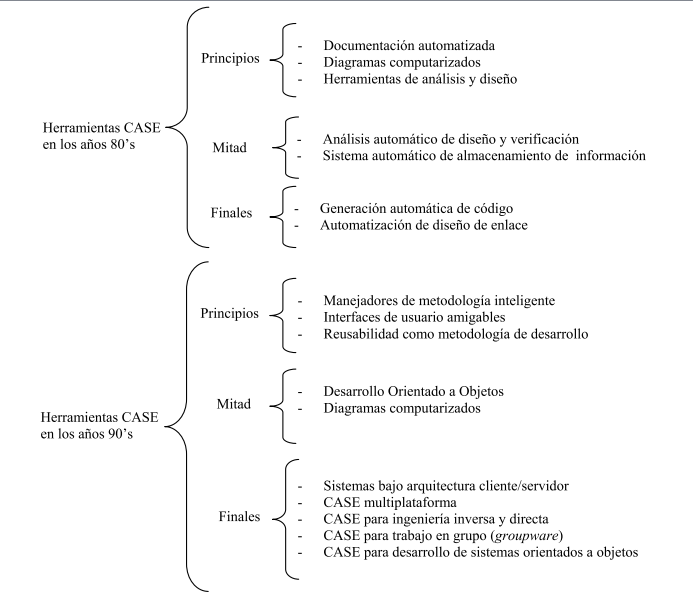
\includegraphics[width=10cm]{figs/case}
  \caption{Historia de las Herramientas CASE}\label{case}
\end{figure}

\subsection{Tipos de CASE}

Seg�n \ac{ONGEI} no existe una �nica clasificaci�n de herramientas CASE y, en ocasiones, es dif�cil incluirlas en una clase determinada. Podr�an clasificarse atendiendo a:

\begin{itemize}
  \item Las plataformas que soportan.
  \item Las fases del ciclo de vida del desarrollo de sistemas que cubren.
  \item La arquitectura de las aplicaciones que producen.
  \item Su funcionalidad.
\end{itemize}

Adem�s seg�n \ac{ONGEI} en funci�n de las fases del ciclo de vida abarcadas,las herramientas CASE se pueden agrupar de la forma siguiente:

\begin{itemize}
  \item Herramientas integradas, I-CASE (Integrated CASE, CASE integrado): abarcan todas las fases del ciclo de vida del desarrollo de sistemas. Son llamadas tambi�n CASE workbench.
  \item Herramienta(s) que comprende(n) alguna(s) fase(s) del ciclo de vida de desarrollo de software:
  \item Herramientas de alto nivel, U-CASE (Upper CASE - CASE superior) o front-end, orientadas a la automatizaci�n y soporte de las actividades desarrolladas durante las primeras fases del desarrollo: an�lisis y dise�o.
  \item Herramientas de bajo nivel, L-CASE (Lower CASE - CASE inferior) o back-end, dirigidas a las �ltimas fases del desarrollo: construcci�n e implantaci�n.
  \item Juegos de herramientas o toolkits, son el tipo m�s simple de herramientas CASE. Automatizan una fase dentro del ciclo de vida. Dentro de este grupo se encontrar�an las herramientas de reingenier�a, orientadas a la fase de mantenimiento.
\end{itemize}

Adem�s seg�n \cite{ONGEI} se puede concluir el siguiente cuadro: \ref{tipoCase}

\begin{figure}
  \centering
  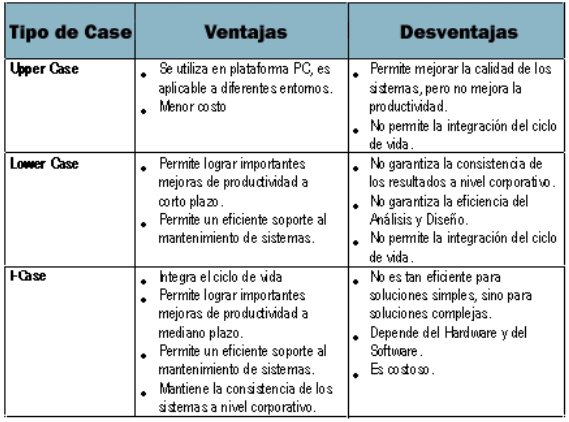
\includegraphics[width=10cm]{figs/tipoCase}
  \caption{Tipos de Case}\label{tipoCase}
\end{figure}

\section{El Lenguaje de Modelado Unificado}

\subsection{Introducci�n}
La Ingenier�a del Software ha tratado con el paso del tiempo simplificar cada vez m�s las complejidades que presentan el an�lisis y dise�o de sistemas de software. Para atacar un problema muy grande es bien sabido que se hace uso de la descomposici�n, para el caso de la Ingenier�a del Software se puede hacer una descomposici�n ya sea algor�tmica
u Orientada a Objetos, d�nde esta �ltima es la de m�s tendencia actualmente.

Debido a esta problem�tica los investigadores de la Ingenier�a del Software han desarrollado diversas metodolog�as Orientadas a Objetos con la finalidad de proporcionar un soporte para los desarrolladores de sistemas para analizar y dise�ar con m�s precisi�n los sistemas. Martin Fowler afirma que actualmente el \ac{UML} es considerado por muchos autores incluyendo a sus creadores James Rumbaugh, Ivar Jacobson y Grady Booch como el lenguaje que unifica los m�todos de An�lisis y Dise�o Orientados a Objetos. \cite{Fowler99}.
\subsubsection{Qu� es el UML}
El \ac{UML} es un lenguaje de modelado gr�fico y visual utilizado para especificar, visualizar, construir y documentar los componentes de un sistema de software. Est� pensado para poder aplicarse en cualquier medio de aplicaci�n que necesite capturar requerimientos y comportamientos del sistema que se desee construir. Ayuda a comprender y a mantener de una mejor forma un sistema basado en un �rea que el analista o desarrollador puede desconocer.

El UML permite captar informaci�n sobre la estructura est�tica y din�mica de un sistema, en donde la estructura est�tica proporciona informaci�n sobre los objetos que intervienen en determinado proceso y las relaciones que existen entre de ellos, y la estructura din�mica define el comportamiento de los objetos a lo largo de todo el tiempo que estos interact�an hasta llegar a su o sus objetivos. \cite{Rumbaugh00}

Una caracter�stica sobresaliente del UML es que no es un m�todo, sino un lenguaje de modelado. Un m�todo define su notaci�n (lenguaje) y su proceso a seguir durante el ciclo de vida de desarrollo del software. El UML s�lo define la notaci�n gr�fica y su significado, a partir de la cual se crear�n los dise�os de sistemas y no depende de un proceso, el cual ser�a el encargado de orientar los pasos a seguir para elaborar el dise�o \cite{Fowler99}.
La idea de usar los diagramas creados mediante el UML es simplemente para mejorar la comunicaci�n, porque ayuda a que los desarrolladores de software se comuniquen con un mismo lenguaje de modelado independiente de las metodolog�as empleadas \cite{Fowler99}.
La ventaja principal del UML \cite{Coleman97} sobre otras notaciones OO es que elimina las diferencias entre sem�nticas y notaciones.
\subsubsection{Antecedentes del UML}
Antes que el UML, hubo muchos intentos por unificar m�todos, el m�s conocido que se se�ala en \cite{Rumbaugh00} es el caso de Fusion por Coleman y sus colegas que incluy� conceptos de los m�todos OMT y Booch , pero como los autores de estos �ltimos no estaban involucrados en la unificaci�n fue tomado como otro m�todo m�s.
El primer acercamiento a UML fue en 1994 cuando se da la noticia de que Jim Rumbaugh se une con Grady Booch en Rational Software Corporation con la finalidad de unificar sus m�todos OMT y Booch respectivamente.
En 1995 sali� a luz la primera propuesta de su m�todo integrado que fue la versi�n 0.8 del entonces llamado M�todo Unificado (Unified Method ). En ese mismo a�o Ivar Jacobson se une a Rational para trabajar con Booch y Rumbaugh en el proceso de unificaci�n, a partir de aqu� a estos tres personajes se les conoce como "Los tres amigos".

En 1996, los tres amigos concluyen su trabajo y lo nombran UML, es entonces cuando el OMG decide convocar a otras compa��as a participar con sus propuestas para mejorar el enfoque est�ndar que el UML pretend�a.

En enero de 1997, todas las propuestas de las empresas � entre las que figuran IBM, Oracle y Rational Software � se unieron en la versi�n 1.0 del UML que fue presentada ante el OMG para su consideraci�n como est�ndar. Y finalmente en Noviembre de 1997 el UML fue adoptado por el OMG y otras organizaciones afines como lenguaje de modelado est�ndar.
En diciembre de 2002 IBM adquiri� las acciones de Rational Software Corporation.

\subsubsection{Conceptos b�sicos}

Como ya se ha mencionado, el \ac{UML} no es un m�todo sino un lenguaje, el cual define �nicamente una notaci�n y un metamodelo  \cite{Fowler99}. El UML al ser un lenguaje est�ndar no depende de un proceso de desarrollo, y esto es precisamente lo que se quer�a al lograr unificar los m�todos, que se tuviera un lenguaje en com�n entre los diferentes m�todos, para que el desarrollador tuviera la libertad de escoger la metodolog�a de su agrado. Con esto los desarrolladores implicados en un proyecto pueden tener la seguridad de que estar�n creando dise�os de software bajo un lenguaje que ser� comprendido por todos aquellos que utilicen el \ac{UML}.

La notaci�n en el UML son los componentes gr�ficos que se utilizan para crear los metamodelos, es decir, es la sintaxis del lenguaje de modelado \cite{Fowler99}. Para el caso de los diagramas de clase, la notaci�n es la forma en c�mo se dibuja una clase, la asociaci�n, la multiplicidad, la agregaci�n, etc.


Un metamodelo o modelo, es la representaci�n de algo en cierta forma, para el caso de la Ingenier�a del Software un modelo es un diagrama que representa la definici�n de la notaci�n.\cite{Fowler99}

\subsection{Las vistas de UML}

Las vistas de UML se refieren a la forma en que se modela una parte del sistema a desarrollar. Los autores del \ac{UML} proponen una clasificaci�n de los diagramas que proporcionan las vistas de \ac{UML}, y aunque pareciera que esta clasificaci�n es algo intuitiva, aclaran que es simplemente una propuesta y que cada desarrollador puede crear su propia clasificaci�n \cite{Schmuller00}. Se muestra la tabla \ref{umlVistas}


\begin{figure}
  \centering
  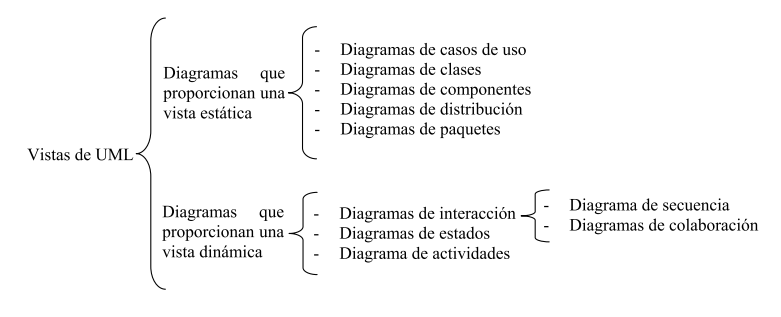
\includegraphics[width=10cm]{figs/umlVistas}
  \caption{Clasificaci�n de vistas y diagramas de UML}\label{umlVistas}
\end{figure}

La vista est�tica es la representaci�n de los elementos del sistema y sus relaciones, la vista din�mica muestra la especificaci�n y la implementaci�n del comportamiento a lo largo del tiempo, es decir muestran el cambio progresivo de los objetos \cite{Rumbaugh00}.

\subsubsection{ Diagramas de Caso de Uso}
Seg�n \cite{Rumbaugh00} La vista que proporcionan los diagramas de casos de uso, modela la forma en c�mo un actor interact�a con el sistema, es decir, describe una interacci�n entre uno o m�s actores y el sistema o subsistemas como una secuencia de mensajes que llevan una forma, tipo y orden. El prop�sito de esta vista es enumerar a los actores y los casos de uso, mostrando un comportamiento y determinar qu� actores participan en cada caso de uso.

La vista de casos de uso es �til para tener una forma de comunicarse con los usuarios finales del sistema, ya que da una visi�n de c�mo ellos esperan que el sistema se comporte.
Un diagrama de casos de uso es una descripci�n l�gica de una parte funcional del sistema y no del sistema en su totalidad. Este diagrama consta de elementos estructurales y relaciones.
\subsubsection{Elementos Estructurales} : Seg�n \cite{Rumbaugh00} y \cite{Schmuller00} los elementos estructurales representan las partes f�sicas o conceptuales de un modelo. La tabla \ref{casoUsoEstructura} muestra estos elementos.
\begin{table}
  \centering
  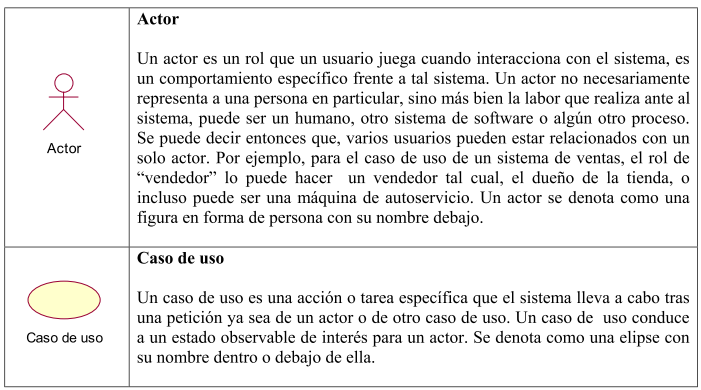
\includegraphics[width=10cm]{figs/casoUsoEstructura}
  \caption{Elementos estructurales de un caso de uso}\label{casoUsoEstructura}
\end{table}

\subsubsection{Relaciones} : Seg�n \cite{Rumbaugh00} y \cite{Schmuller00} las relaciones conectan a los elementos estructurales para darles sentido al diagrama de casos de uso. La tabla \ref{casoUsoRelacion} muestra estas relaciones.
\begin{table}
  \centering
  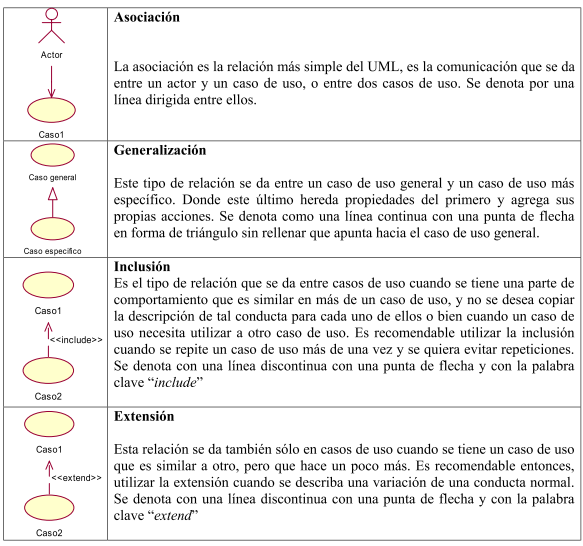
\includegraphics[width=10cm]{figs/casoUsoRelacion}
  \caption{Relaciones dentro de un caso de uso}\label{casoUsoRelacion}
\end{table}

\subsection{Diagrama de Clases}

Seg�n \cite{Rumbaugh00} y \cite{Schmuller00} la vista de los diagramas de clase, visualiza las relaciones entre las clases que se involucran en el sistema. Un diagrama de clases muestra un conjunto de clases, interfaces y colaboraciones y las relaciones entre �stas, mostrando as�, la estructura est�tica de un sistema. Los diagramas de clase pueden mostrar:

\begin{itemize}
  \item Clases
  \item Atributos
  \item Operaciones
  \item Asociaciones
  \item Generalizaciones
  \item Agregaciones
  \item Composiciones
\end{itemize}
Un diagrama de clases esta compuesto por los elementos mostrados en las tablas \ref{clase1} y \ref{clase2}.

\begin{table}
  \centering
  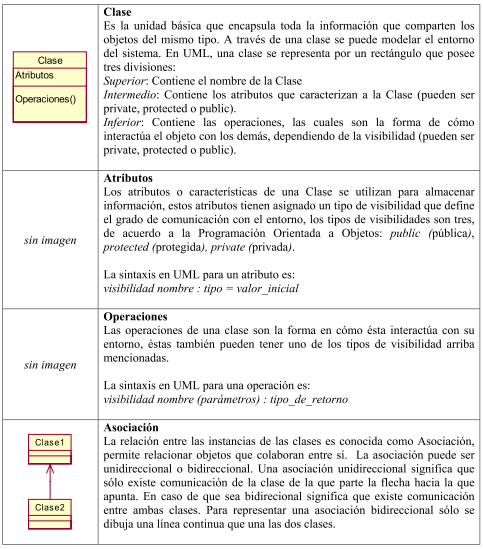
\includegraphics[width=10cm]{figs/clase1}
  \caption{Relaciones dentro de un caso de uso}\label{clase1}
\end{table}
\begin{table}
  \centering
  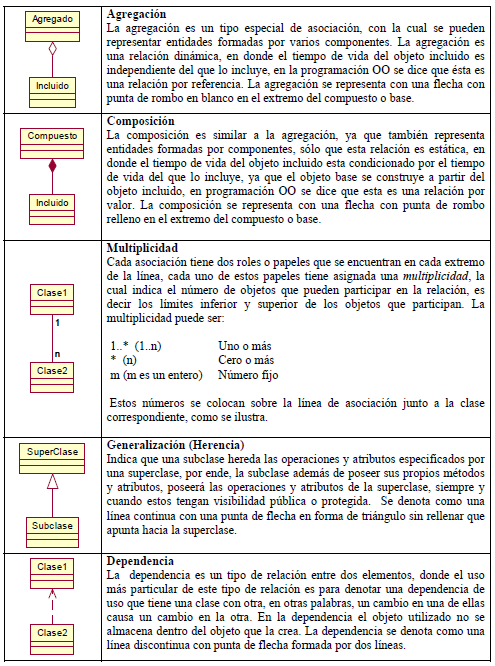
\includegraphics[width=10cm]{figs/clase2}
  \caption{Relaciones dentro de un caso de uso}\label{clase2}
\end{table}


\section{Patr�n DAO}
Seg�n \cite{Gamma03}, "cada patr�n describe un problema que ocurre una y otra vez en nuestro entorno, as� como soluci�n a ese problema,de tal modo que se pueda aplicar esta soluci�n un mill�n de veces, sin hacer lo mismo dos veces"
En general un patr�n tiene cuatro elementos esenciales:
\begin{itemize}
  \item EL nombre del patr�n que permite describir, en una o dos palabras, un problema de dise�o junt con sus soluciones y consecuencias.
  \item El problema Describe cuando aplicar el patr�n. Explica el problema y su context. Puede describir problemas concretos de dise�o as� como las estructuras de clases u objetos que son sintom�ticas de un dise�o inflexible. A veces el problema incluye una serie de condiciones que deben darse para que tenga sentido aplicar el patr�n
  \item La soluci�n, que describe los elementos que constituyen el dise�o, sus relaciones, responsabilidades y colaboraciones.
  \item Las consecuencias son los resultados as� como las ventajase inconvenientes de aplicar el patr�n.
\end{itemize}

Seg�n \cite{Gamma03}, es bastante normal hacer aplicaciones que almacenan y recogen datos de una base de datos. Suele ser habitual, tambi�n, querer hacer nuestra aplicaci�n lo m�s independiente posible de una base de datos concreta, de c�mo se accede a los datos o incluso de si hay o no base de datos detr�s. Nuestra aplicaci�n debe conseguir los datos o ser capaz de guardarlos en alg�n sitio, pero no tiene por qu� saber de d�nde los est� sacando o d�nde se guardan.
Hay una forma de hacer esto que ha resultado bastante eficiente en el mundo JEE y de aplicaciones web, pero que es aplicable a cualquier tipo de aplicaci�n que deba recoger datos de alg�n sitio y almacenarlos. Es lo que se conoce como patr�n DAO (Data Access Object).
La idea de este patr�n es sencilla. En primer lugar, debemos hacernos las clases que representan nuestros datos. Por ejemplo, podemos hacer una clase Persona con los datos de la persona y los m�todos set() y get() correspondientes.
Luego hacemos una interface. Esta interface tiene que tener los m�todos necesarios para obtener y almacenar Personas. Esta interface no debe tener nada que la relaciones con una base de datos ni cualquier otra cosa espec�fica del medio de almacenamiento que vayamos a usar, es decir, ning�n par�metro deber�a ser una Connection, ni un nombre de fichero, etc.

 %Inserta el cap�tulo 2
%\chapter{Estado del Arte}\label{chap:estadodelarte}

Objetivo: El informe del estado del arte permite evaluar el nivel de conocimiento del candidato respecto del problema que desea resolver. El estado del arte describe todo aquello que otros investigadores han estudiado acerca del problema. La redacci�n de la misma corresponde a uno o dos cap�tulos del informe final de su tesis

Consideraciones: El estado del arte est� conformado por la definici�n del problema, las variaciones del problema (si existiera), la taxonom�a (en donde se encuentra el problema de estudio), las metodolog�as, modelos, algoritmos, aplicaciones, aplicativos (software), plataformas asociados directamente al problema, esto es, aplicado al problema de estudio.
No se debe confundir el estado del arte con el marco te�rico. El estado del arte se centra al  problema de estudio. Entretanto el marco te�rico es dado por los fundamentos alrededor del tema de tesis

Estructura del informe: La estructura del estado del arte debe incluir en lo posible:
�	Taxonom�a (variantes o clasificaci�n del problema)
�	M�todos / Modelos / Procedimientos / Buenas Pr�cticas
�	Algoritmos
�	Aplicativos/ Arquitecturas/ Software
�	Casos de estudios/ aplicaciones
�	Marco legal/ Normas/ / Regulaciones
Taxonom�a: La taxonom�a consiste en la clasificaci�n del problema, y tiene por objetivo que el lector tenga un panorama mayor sobre el problema en estudio. Algunas veces no es posible hacer una taxonom�a.
Aplicaciones: Describir las diversas aplicaciones (uso) existentes en la literatura. Por ejemplo, el tema �algoritmos gen�ticos para la optimizaci�n de cortes en una dimensi�n�, tiene diversas aplicaciones como: cortes de fierros, cortes de aluminio, cortes de bobina de papel, etc.
M�todos / Modelos / Buenas Pr�cticas: Describir sucintamente Deber� ser presentado los diversos m�todos/ modelos/ Buenas pr�cticas que han sido desarrollado para resolver el problema en estudio.
Aplicativos (software): Describir los diversos software que existen en la literatura y en el �mbito comercial. Se�alar las bondades, restricciones, y el m�todo en la implementaci�n del software (si lo hubiera).
 %Inserta el cap�tulo 3
\chapter{Aporte Metodol�gico}\label{chap:metodologia}
 %Inserta el cap�tulo 4

%%%%%%%%%%%%%%%%%%%%%%%%%%%%%%%%%%%%%%%%%%%%%%%%%%%%%%%%%%%%%%%%%%%%%%

\bibliographystyle{plain}
\bibliography{Bibliog}
\addcontentsline{toc}{chapter}{Bibliograf\'ia}
\end{document}
